\documentclass[11pt,letterpaper]{article}

\usepackage[utf8]{inputenc}
\usepackage[T1]{fontenc}
\usepackage{lmodern}
\usepackage[spanish,es-noquoting]{babel}
\usepackage[left=2.4cm,right=2.4cm,top=2.6cm,bottom=2.4cm]{geometry}
\usepackage{amsmath,amssymb}
\usepackage{booktabs}
\usepackage{longtable}
\usepackage{array}
\usepackage{graphicx}
\usepackage{float}
\usepackage{pdflscape}
\usepackage{xcolor}
\usepackage{caption}
\usepackage{enumitem}
\usepackage{microtype}
\usepackage{setspace}
\usepackage{fancyhdr}
\usepackage[colorlinks=true,linkcolor=black,urlcolor=blue!55!black]{hyperref}
\hypersetup{pdftitle={Proyecto Convocatoria 2 - Analisis Sintactico - AgroRule (INFO1148)},
            pdfauthor={Nicolas Vergara Von dem Knesebeck, Rodrigo Altamirano Leon},
            pdfsubject={Teoria de la Computacion - INFO1148 - UCT},
            pdfkeywords={analisis sintactico, LL(1), FIRST, FOLLOW, gramatica libre de contexto, DSL}}

\setlength{\parskip}{0.5em}
\setlength{\parindent}{0pt}
\setlength{\emergencystretch}{2em}
\renewcommand{\arraystretch}{1.15}
\captionsetup{font=small,labelfont=bf}
\onehalfspacing

\newcommand{\code}[1]{\texttt{#1}}
\newcommand{\dq}{\textquotedbl{}}
\newcolumntype{L}[1]{>{\raggedright\arraybackslash}p{#1}}
\newcolumntype{C}[1]{>{\centering\arraybackslash}p{#1}}

\pagestyle{fancy}
\fancyhf{}
\fancyhead[L]{\small Teoría de la Computación -- INFO1148}
\fancyhead[R]{\small Proyecto: analizador sintáctico}
\fancyfoot[C]{\thepage}
\renewcommand{\headrulewidth}{0.4pt}

\begin{document}

\begin{titlepage}
\centering
\vspace*{2.4cm}
{\small UNIVERSIDAD CATÓLICA DE TEMUCO \quad|\quad FACULTAD DE INGENIERÍA}\\[2pt]
{\small Ingeniería Civil en Informática}\\[14pt]
\rule{\textwidth}{0.6pt}\\[10pt]
{\Large\bfseries Teoría de la Computación -- INFO1148}\\[12pt]
{\large Proyecto: diseño e implementación de un analizador sintáctico\\[2pt]Convocatoria 2}\\[10pt]
{\large\bfseries AgroRule: lenguaje de dominio específico\\ para la automatización de un invernadero}\\[10pt]
{\small Informe técnico y código fuente}\\[18pt]
\rule{\textwidth}{0.6pt}\\[16pt]

\begin{tabular}{rl}
\textbf{Estudiantes} & Nicolás Vergara Von dem Knesebeck (jefe de grupo)\\
                     & Rodrigo Altamirano León\\[6pt]
\textbf{Profesor}    & Marcos Antonio Levano Huamaccto\\
\textbf{Curso}       & INFO1148 -- 2026-2\\
\textbf{Fecha}       & 15 de noviembre de 2026\\
\end{tabular}

\vfill
{\footnotesize Repositorio del proyecto: \url{https://github.com/objval/agrorule-info1148/tree/convocatoria-2}}
\end{titlepage}

\begingroup
\renewcommand{\contentsname}{Índice}
\small
\setlength{\parskip}{0pt}
\tableofcontents
\endgroup
\newpage

\section{Introducción y dominio seleccionado}

Un invernadero automatizado recibe lecturas de sensores (temperatura, humedad de suelo, humedad ambiental, luz, pH, lluvia) y actúa sobre mecanismos (riego, ventiladores, mallas, techo, calefacción). La lógica que une unas con otros suele escribirse como reglas del tipo ``si pasa esto, haz aquello''. En la práctica esas reglas terminan dentro del código de un controlador, mezcladas con la lectura de sensores, y cualquier cambio de criterio obliga a modificar y volver a desplegar el programa completo.

Este proyecto define un lenguaje de dominio específico para escribir esas reglas por separado y un analizador sintáctico que verifica que estén bien escritas antes de que el controlador las ejecute. El lenguaje se llama \textbf{AgroRule}. El alcance del proyecto es el análisis sintáctico, no la ejecución de las reglas, y por eso el resultado del analizador es un árbol sintáctico abstracto y no una secuencia de acciones ejecutadas.

El dominio se eligió por tres razones. Primero, las reglas de un invernadero se parecen mucho entre sí, lo que permite una gramática pequeña y un lenguaje que se aprende en minutos. Segundo, el vocabulario es concreto y verificable, con magnitudes físicas y actuadores reconocibles. Tercero, el lenguaje necesita condiciones compuestas, porque casi ninguna decisión agronómica depende de una sola variable. Esa necesidad obliga a resolver precedencia, asociatividad y anidamiento, que es justamente el contenido del curso.

\section{Especificación del lenguaje}

\subsection{Alfabeto y categorías de tokens}

El alfabeto del lenguaje incluye letras, dígitos, el guion bajo, los operadores relacionales, los paréntesis, la coma, el punto y coma, las comillas y el símbolo de comentario. El analizador léxico agrupa esos caracteres en las categorías de la Tabla~\ref{tab:tokens}.

\begin{table}[htbp]
\centering
\caption{Categorías de tokens de AgroRule.}
\label{tab:tokens}
\small
\begin{tabular}{L{2.6cm}L{5.4cm}L{7.4cm}}
\toprule
\textbf{Categoría} & \textbf{Ejemplos} & \textbf{Descripción} \\
\midrule
Palabras reservadas & \code{WHEN}, \code{THEN}, \code{AND}, \code{OR}, \code{NOT}, \code{END}, \code{TRUE}, \code{FALSE} & Ocho palabras con significado fijo, escritas en mayúsculas \\
Identificador & \code{temperatura}, \code{abrir\_ventilador}, \code{ph\_suelo} & Letra o guion bajo seguido de letras, dígitos o guion bajo \\
Número & \code{28}, \code{6.5}, \code{1.5} & Entero o decimal con punto \\
Booleano & \code{TRUE}, \code{FALSE} & Valor de verdad, se comporta como palabra reservada \\
Texto & \code{\dq calor\dq}, \code{\dq nitrato\dq} & Cadena entre comillas dobles, sin salto de línea \\
Operador relacional & \code{>}, \code{<}, \code{>=}, \code{<=}, \code{==}, \code{!=} & Compara dos términos \\
Paréntesis & \code{(}, \code{)} & Agrupan condiciones \\
Separadores & \code{;}, \code{,} & Separan acciones y argumentos \\
Comentario & \code{\# texto} & Se ignora hasta el final de la línea \\
\bottomrule
\end{tabular}
\end{table}

Cada token conserva la línea y la columna donde empieza. Esa decisión no es cosmética: todos los mensajes de error del sistema apuntan a una posición concreta de la entrada, y sin esa información el usuario solo sabría que algo está mal, no dónde. Los números usan dígitos ASCII, exigen al menos un dígito a cada lado del punto decimal y su conversión a coma flotante debe ser finita. Las palabras reservadas distinguen mayúsculas de minúsculas. \code{when} no equivale a \code{WHEN}.

\subsection{Forma de una regla}

Una regla tiene cuatro partes. La palabra \code{WHEN} abre la regla, una condición indica cuándo se aplica, \code{THEN} separa la condición de las acciones y \code{END} cierra la regla. Dentro de la condición se comparan dos términos con un operador relacional, y esas comparaciones se pueden unir con \code{AND}, \code{OR}, negar con \code{NOT} y agrupar con paréntesis. Las acciones son identificadores que pueden llevar argumentos entre paréntesis y se separan con punto y coma. Un programa es una secuencia de reglas.

\subsection{Ejemplos de sentencias}

\begin{table}[htbp]
\centering
\caption{Cinco sentencias válidas y cinco inválidas del lenguaje.}
\label{tab:ejemplos}
\footnotesize
\begin{tabular}{L{0.7cm}L{9.3cm}L{5.4cm}}
\toprule
\textbf{N} & \textbf{Sentencia} & \textbf{Comentario} \\
\midrule
V1 & \code{WHEN temperatura > 28 THEN abrir\_ventilador END} & Regla mínima \\
V2 & \code{WHEN humedad < 30 AND temperatura > 25 THEN regar(20) END} & Condición compuesta con AND \\
V3 & \code{WHEN NOT (temperatura > 30) THEN cerrar\_techo END} & Negación de un grupo \\
V4 & \code{WHEN ph >= 6.5 AND ph <= 7.5 THEN fertirriego(1.5, \dq nitrato\dq) END} & Argumento numérico y de texto \\
V5 & \code{WHEN suelo == seco OR lluvia == FALSE THEN regar(15); avisar(\dq riego\dq) END} & Dos acciones en una regla \\
\midrule
I1 & \code{WHEN temperatura > 28 abrir\_ventilador END} & Falta THEN \\
I2 & \code{WHEN temperatura > 28 THEN abrir\_ventilador} & Falta END \\
I3 & \code{WHEN temperatura > THEN regar(20) END} & Falta el valor de la derecha \\
I4 & \code{WHEN temperatura > 28 THEN regar(20) abrir\_ventilador END} & Falta el punto y coma entre acciones \\
I5 & \code{WHEN temperatura 28 THEN regar(20) END} & Falta el operador relacional \\
\bottomrule
\end{tabular}
\end{table}

\section{Gramática libre de contexto}

\subsection{Símbolo inicial, terminales y no terminales}

La gramática se define sobre el conjunto de tokens, no sobre caracteres, porque el analizador léxico ya resolvió esa parte. El símbolo inicial es \code{programa}. La gramática tiene 19 no terminales, 16 símbolos terminales y el centinela de fin de entrada (\$). Los no terminales con apóstrofo (\code{disy'}, \code{conj'}, \code{acciones'}, \code{args'}) representan la repetición de una estructura y existen para evitar la recursión izquierda.

\subsection{Producciones}

{\small\begin{longtable}{L{1.1cm}L{12.2cm}}
\caption{Producciones de la gramática de AgroRule.}\label{tab:producciones}\\
\toprule\textbf{ID}&\textbf{Producción}\\\midrule\endfirsthead
\toprule\textbf{ID}&\textbf{Producción}\\\midrule\endhead
P1&programa $\rightarrow$ lista\_reglas\\
P2&lista\_reglas $\rightarrow$ regla lista\_reglas\\
P3&lista\_reglas $\rightarrow$ $\varepsilon$\\
P4&regla $\rightarrow$ WHEN cond THEN acciones END\\
P5&cond $\rightarrow$ disy\\
P6&disy $\rightarrow$ conj disy'\\
P7&disy' $\rightarrow$ OR conj disy'\\
P8&disy' $\rightarrow$ $\varepsilon$\\
P9&conj $\rightarrow$ neg conj'\\
P10&conj' $\rightarrow$ AND neg conj'\\
P11&conj' $\rightarrow$ $\varepsilon$\\
P12&neg $\rightarrow$ NOT neg\\
P13&neg $\rightarrow$ prim\\
P14&prim $\rightarrow$ LPAREN cond RPAREN\\
P15&prim $\rightarrow$ comp\\
P16&comp $\rightarrow$ term OP\_REL term\\
P17&term $\rightarrow$ IDENT\\
P18&term $\rightarrow$ NUM\\
P19&term $\rightarrow$ TRUE\\
P20&term $\rightarrow$ FALSE\\
P21&acciones $\rightarrow$ accion acciones'\\
P22&acciones' $\rightarrow$ SEMI accion acciones'\\
P23&acciones' $\rightarrow$ $\varepsilon$\\
P24&accion $\rightarrow$ IDENT llamada\\
P25&llamada $\rightarrow$ LPAREN args RPAREN\\
P26&llamada $\rightarrow$ $\varepsilon$\\
P27&args $\rightarrow$ arg args'\\
P28&args' $\rightarrow$ COMMA arg args'\\
P29&args' $\rightarrow$ $\varepsilon$\\
P30&arg $\rightarrow$ NUM\\
P31&arg $\rightarrow$ TRUE\\
P32&arg $\rightarrow$ FALSE\\
P33&arg $\rightarrow$ IDENT\\
P34&arg $\rightarrow$ CADENA\\
\bottomrule\end{longtable}}


La gramática tiene 34 producciones. Las reglas auxiliares expresan la repetición de condiciones, acciones y argumentos sin recursión izquierda. El orden de las producciones no influye en el análisis, porque el parser decide por token de adelanto y no por orden de escritura.

\section{Análisis de la gramática}

\subsection{Recursión izquierda}

La gramática no tiene recursión izquierda. El caso crítico son las condiciones compuestas: si se escribiera \code{disy $\rightarrow$ disy OR conj}, el analizador de descenso recursivo llamaría a \code{disy} con la misma entrada y entraría en un ciclo infinito. Para evitarlo, la repetición se expresa con un no terminal auxiliar a la derecha, como en \code{disy $\rightarrow$ conj disy'} y \code{disy' $\rightarrow$ OR conj disy' $\mid \varepsilon$}. Esa forma produce una asociatividad por la izquierda en el árbol resultante sin recursión por la izquierda en la gramática.

\subsection{Factorización por la izquierda}

Hay un solo lugar donde la factorización fue necesaria. Con las producciones \code{accion $\rightarrow$ IDENT args} y \code{accion $\rightarrow$ IDENT} el parser no podría decidir cuál aplicar mirando un identificador, porque ambas empiezan con el mismo símbolo. La solución fue sacar el prefijo común: \code{accion $\rightarrow$ IDENT llamada} y \code{llamada $\rightarrow$ ( args ) $\mid \varepsilon$}. Ahora la decisión se toma después de leer el identificador, cuando el siguiente token es un paréntesis o no lo es.

\subsection{Ambigüedad}

La gramática no es ambigua. La precedencia entre \code{AND} y \code{OR} no se deja al azar ni a una convención implícita: está en la estructura de la gramática. El no terminal \code{disy} agrupa conjunciones y el no terminal \code{conj} agrupa negaciones, de modo que \code{AND} se resuelve antes que \code{OR} y los paréntesis permiten alterar ese orden. Una gramática plana del tipo \code{cond $\rightarrow$ cond AND cond $\mid$ cond OR cond} sería ambigua y además recursiva por la izquierda.

El caso de las acciones se resolvió de forma parecida. Cada acción termina en un punto y coma o en \code{END}, y esos dos símbolos no aparecen dentro de una acción, así que el límite entre acciones nunca es ambiguo.

\subsection{Conjuntos FIRST y FOLLOW}

{\small\setlength{\tabcolsep}{4pt}\begin{longtable}{L{2.8cm}L{6.3cm}L{5.9cm}}
\caption{Conjuntos FIRST y FOLLOW por no terminal.}\label{tab:firstfollow}\\
\toprule\textbf{No terminal}&\textbf{FIRST}&\textbf{FOLLOW}\\\midrule\endfirsthead
\toprule\textbf{No terminal}&\textbf{FIRST}&\textbf{FOLLOW}\\\midrule\endhead
programa&{WHEN, $\varepsilon$}&{\$}\\
lista\_reglas&{WHEN, $\varepsilon$}&{\$}\\
regla&{WHEN}&{WHEN, \$}\\
cond&{NOT, (, id, num, TRUE, FALSE}&{THEN, )}\\
disy&{NOT, (, id, num, TRUE, FALSE}&{THEN, )}\\
disy'&{OR, $\varepsilon$}&{THEN, )}\\
conj&{NOT, (, id, num, TRUE, FALSE}&{THEN, OR, )}\\
conj'&{AND, $\varepsilon$}&{THEN, OR, )}\\
neg&{NOT, (, id, num, TRUE, FALSE}&{THEN, OR, AND, )}\\
prim&{(, id, num, TRUE, FALSE}&{THEN, OR, AND, )}\\
comp&{id, num, TRUE, FALSE}&{THEN, OR, AND, )}\\
term&{id, num, TRUE, FALSE}&{THEN, OR, AND, ), op}\\
acciones&{id}&{END}\\
acciones'&{;, $\varepsilon$}&{END}\\
accion&{id}&{END, ;}\\
llamada&{(, $\varepsilon$}&{END, ;}\\
args&{id, num, TRUE, FALSE, txt}&{)}\\
args'&{,, $\varepsilon$}&{)}\\
arg&{id, num, TRUE, FALSE, txt}&{), ,}\\
\bottomrule\end{longtable}}


Dos conjuntos explican por qué la gramática es LL(1). FIRST de \code{cond} es $\{$\code{NOT}, \code{(}, \code{id}, \code{num}, \code{TRUE}, \code{FALSE}$\}$ porque una condición puede empezar con una negación, con un paréntesis o directamente con una comparación. FOLLOW de \code{disy'} es $\{$\code{THEN}, \code{)}$\}$, porque un \code{disy'} termina cuando aparece \code{THEN} o el paréntesis que cierra la condición que lo contiene. Esos dos conjuntos no se cruzan con FIRST de la otra alternativa de \code{disy'}, que es $\{$\code{OR}$\}$, y por eso la decisión es única.

\subsection{Verificación LL(1)}

La tabla predictiva se construyó con un algoritmo que, para cada producción, calcula su conjunto de predicción y detecta si dos producciones del mismo no terminal compiten por el mismo terminal. El resultado fue cero conflictos. La comprobación no es una revisión manual: el mismo cálculo que genera la tabla del informe es el que usa el analizador en tiempo de ejecución, y una prueba automática falla si aparece un conflicto nuevo.

\section{Tabla LL(1)}

La Tabla~\ref{tab:ll1} se presenta en orientación horizontal porque tiene diecisiete columnas. Cada celda indica la producción que el analizador aplica cuando el no terminal de la fila aparece con el token de la columna en la entrada. Las celdas vacías representan combinaciones que la gramática no admite, y son las que generan los mensajes de error.

La lectura de la tabla es directa. En la fila \code{programa} se aplica P1 tanto con \code{WHEN} como con el centinela \$, porque la lista de reglas admite un programa vacío. En la fila \code{regla} todas las celdas están vacías salvo \code{WHEN}, lo que confirma que una regla no puede empezar de otra forma. En la fila \code{neg} aparecen dos alternativas, P12 con \code{NOT} y P13 con los símbolos que pueden iniciar una condición primaria. Esta separación permite leer \code{NOT NOT} sin ambigüedad.

Hay dos filas que conviene mirar juntas. \code{disy'} solo tiene P7 en la columna \code{OR} y P8 en \code{THEN} y \code{)}, mientras \code{conj'} tiene P10 en \code{AND} y P11 en \code{THEN}, \code{OR} y \code{)}. La diferencia entre ambas filas es exactamente la precedencia: \code{OR} cierra una conjunción pero no al revés, y por eso \code{a > 1 OR b > 2 AND c > 3} se agrupa como se espera.

La tabla también explica el comportamiento del analizador frente a un error. Cuando la celda correspondiente está vacía, el parser no elige una producción al azar ni intenta retroceder: informa los símbolos que la fila sí admitía. Un \code{then} que aparece antes de cerrar la condición produce un mensaje con \code{AND}, \code{OR} y el paréntesis de cierre como alternativas, porque esas son las columnas ocupadas de la fila \code{conj'}.

\begin{landscape}
\thispagestyle{empty}
{\scriptsize\setlength{\tabcolsep}{3.4pt}\begin{longtable}{L{1.7cm}C{0.98cm}C{0.98cm}C{0.98cm}C{0.98cm}C{0.98cm}C{0.98cm}C{0.98cm}C{0.98cm}C{0.98cm}C{0.98cm}C{0.98cm}C{0.98cm}C{0.98cm}C{0.98cm}C{0.98cm}C{0.98cm}C{0.98cm}}
\caption{Tabla predictiva LL(1). Cada celda indica la producción que se aplica.}\label{tab:ll1}\\
\toprule\textbf{No terminal}&\rotatebox{90}{\scriptsize WHEN}&\rotatebox{90}{\scriptsize THEN}&\rotatebox{90}{\scriptsize END}&\rotatebox{90}{\scriptsize OR}&\rotatebox{90}{\scriptsize AND}&\rotatebox{90}{\scriptsize NOT}&\rotatebox{90}{\scriptsize (}&\rotatebox{90}{\scriptsize )}&\rotatebox{90}{\scriptsize op}&\rotatebox{90}{\scriptsize id}&\rotatebox{90}{\scriptsize num}&\rotatebox{90}{\scriptsize TRUE}&\rotatebox{90}{\scriptsize FALSE}&\rotatebox{90}{\scriptsize ;}&\rotatebox{90}{\scriptsize ,}&\rotatebox{90}{\scriptsize txt}&\rotatebox{90}{\scriptsize \$}\\\midrule\endfirsthead
\toprule\textbf{No terminal}&\rotatebox{90}{\scriptsize WHEN}&\rotatebox{90}{\scriptsize THEN}&\rotatebox{90}{\scriptsize END}&\rotatebox{90}{\scriptsize OR}&\rotatebox{90}{\scriptsize AND}&\rotatebox{90}{\scriptsize NOT}&\rotatebox{90}{\scriptsize (}&\rotatebox{90}{\scriptsize )}&\rotatebox{90}{\scriptsize op}&\rotatebox{90}{\scriptsize id}&\rotatebox{90}{\scriptsize num}&\rotatebox{90}{\scriptsize TRUE}&\rotatebox{90}{\scriptsize FALSE}&\rotatebox{90}{\scriptsize ;}&\rotatebox{90}{\scriptsize ,}&\rotatebox{90}{\scriptsize txt}&\rotatebox{90}{\scriptsize \$}\\\midrule\endhead
programa&P1&&&&&&&&&&&&&&&&P1\\
lista\_reglas&P2&&&&&&&&&&&&&&&&P3\\
regla&P4&&&&&&&&&&&&&&&&\\
cond&&&&&&P5&P5&&&P5&P5&P5&P5&&&&\\
disy&&&&&&P6&P6&&&P6&P6&P6&P6&&&&\\
disy'&&P8&&P7&&&&P8&&&&&&&&&\\
conj&&&&&&P9&P9&&&P9&P9&P9&P9&&&&\\
conj'&&P11&&P11&P10&&&P11&&&&&&&&&\\
neg&&&&&&P12&P13&&&P13&P13&P13&P13&&&&\\
prim&&&&&&&P14&&&P15&P15&P15&P15&&&&\\
comp&&&&&&&&&&P16&P16&P16&P16&&&&\\
term&&&&&&&&&&P17&P18&P19&P20&&&&\\
acciones&&&&&&&&&&P21&&&&&&&\\
acciones'&&&P23&&&&&&&&&&&P22&&&\\
accion&&&&&&&&&&P24&&&&&&&\\
llamada&&&P26&&&&P25&&&&&&&P26&&&\\
args&&&&&&&&&&P27&P27&P27&P27&&&P27&\\
args'&&&&&&&&P29&&&&&&&P28&&\\
arg&&&&&&&&&&P33&P30&P31&P32&&&P34&\\
\bottomrule\end{longtable}}

\end{landscape}

\section{Diseño e implementación del parser}

\subsection{Estructura del código}

El código está separado en módulos con una responsabilidad cada uno. La Tabla~\ref{tab:modulos} resume esa separación.

\begin{table}[htbp]
\centering
\caption{Módulos del analizador y su responsabilidad.}
\label{tab:modulos}
\small
\begin{tabular}{L{3.4cm}L{11.6cm}}
\toprule
\textbf{Módulo} & \textbf{Responsabilidad} \\
\midrule
\code{lexer.py} & Convierte el texto en tokens con línea y columna. Reconoce comentarios, números, textos e identificadores \\
\code{grammar.py} & Declara las producciones una sola vez y calcula FIRST, FOLLOW, la tabla LL(1) y los conflictos \\
\code{parser.py} & Analizador por descenso recursivo. Una función por no terminal, decisión por tabla \\
\code{ast\_nodes.py} & Nodos del árbol, dibujo en texto y exportación a Graphviz \\
\code{errors.py} & Errores léxicos y sintácticos con posición, símbolo esperado y símbolo encontrado \\
\code{cli.py} & Interfaz de línea de comandos con opciones para árbol, tokens, tabla y exportación \\
\bottomrule
\end{tabular}
\end{table}

No se usó ningún generador de analizadores. La gramática se declara como una lista de tuplas y los algoritmos de FIRST, FOLLOW y tabla predictiva están escritos en el mismo módulo, con unas cien líneas en total.

\subsection{Cómo se usa la tabla en el parser}

Cada función del parser corresponde a un no terminal. Cuando ese no terminal tiene más de una producción, la función no decide con una cadena de condicionales sobre el texto: consulta \code{TABLA[no\_terminal][token.tipo]} y aplica la producción que la tabla indica. Si la celda está vacía, el error se construye con la lista de tokens que la tabla sí admitía en esa fila.

Esa decisión tiene una consecuencia práctica. El mensaje de error y la gramática no pueden desincronizarse, porque ambos salen de la misma estructura. Si mañana se agrega una producción, la tabla se recalcula y los mensajes de error incluyen el símbolo nuevo sin tocar el manejador de errores.

\subsection{Complejidad y comportamiento}

El analizador recorre la entrada con un token de adelanto y sin retroceder. El costo es lineal en la cantidad de tokens. Las negaciones consecutivas se procesan iterativamente. Los paréntesis anidados conservan el descenso recursivo, con un límite de 80 grupos: a partir del siguiente se devuelve un error sintáctico con línea y columna. Las pruebas comprueban 40 grupos válidos y el rechazo controlado de 81.

\section{Árbol sintáctico}

El resultado del análisis es un árbol sintáctico abstracto. La diferencia con un árbol de derivación es deliberada: el árbol de derivación conserva cada paso de la gramática, incluidos \code{WHEN}, \code{THEN} y \code{END}, mientras que el AST conserva solo la estructura semántica. Un \code{AND} queda como un nodo con dos hijos, una comparación como un nodo con operador y dos términos, y una acción como un nodo con nombre y argumentos.

\begin{figure}[htbp]
\centering
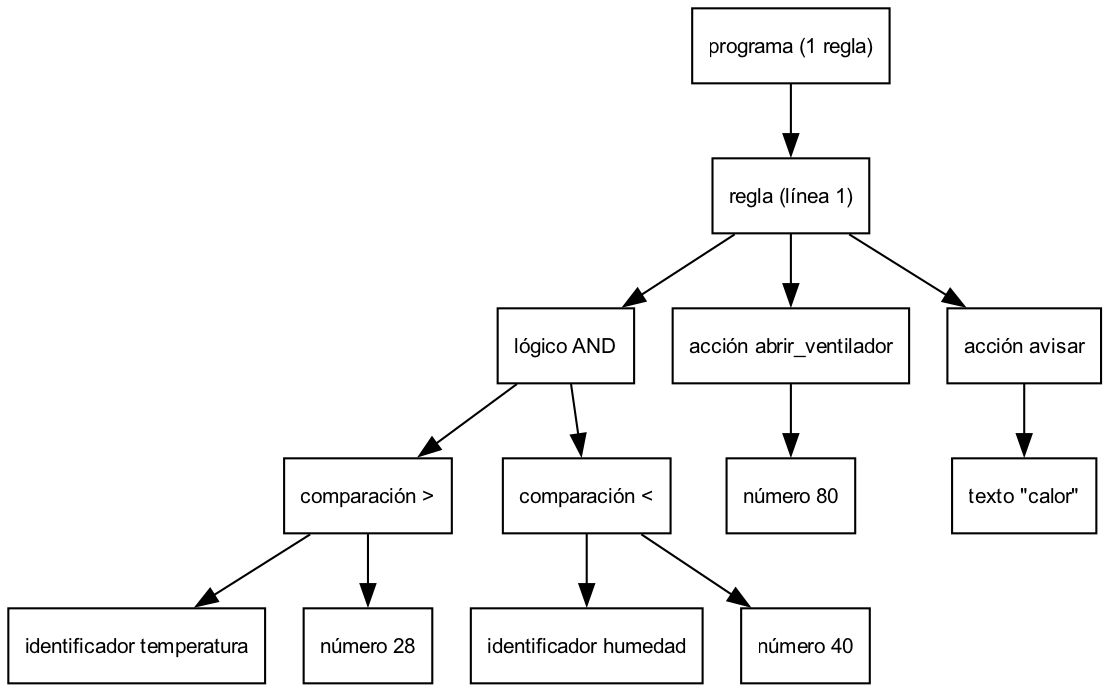
\includegraphics[width=0.86\textwidth]{figuras/ast.png}
\caption{AST generado para \code{WHEN temperatura > 28 AND humedad < 40 THEN abrir\_ventilador(80); avisar(\dq calor\dq) END}.}
\label{fig:ast}
\end{figure}

La Figura~\ref{fig:ast} muestra la estructura del árbol: \code{AND} agrupa dos comparaciones y las acciones cuelgan de la regla en el orden escrito. La ejecución del analizador y un rechazo con error localizado se documentan con capturas en el Anexo~\ref{sec:demo}.

\section{Manejo de errores}

El analizador distingue tres familias de error. La primera es léxica y aparece cuando hay un carácter que no pertenece al alfabeto o un texto sin cerrar. La segunda es sintáctica y aparece cuando la secuencia de tokens no corresponde a ninguna producción aplicable. La tercera es de fin de entrada, cuando el programa termina antes de cerrar una regla o una lista de argumentos.

Todos los mensajes incluyen línea, columna y una explicación en palabras del dominio. Algunos ejemplos reales de salida son los siguientes.

\begin{quote}
\small\ttfamily\raggedright
Error sintáctico (línea 1, columna 23): se esperaba AND, OR o el final de la condición (THEN o un paréntesis de cierre). Se esperaba: AND, OR, ), THEN. Se encontró: identificador.

Error sintáctico (línea 1, columna 20): se esperaba un valor (número, identificador, TRUE o FALSE). Se esperaba: FALSE, identificador, número, TRUE. Se encontró: THEN.

Error sintáctico (línea 1, columna 38): se esperaba ';' entre acciones o END para cerrar la regla. Se esperaba: END, ;. Se encontró: identificador.

Error léxico (línea 1, columna 42): carácter no permitido: '@'.
\end{quote}

El mensaje no se limita a decir que hay un error. Indica qué construcción se estaba leyendo, qué símbolos habrían permitido continuar y qué símbolo apareció. La captura del Anexo~\ref{sec:demo} muestra un rechazo por ausencia de \code{THEN}.

\section{Casos de prueba}

La Tabla~\ref{tab:casos} se generó ejecutando el analizador sobre cada entrada. Muestra por separado la aceptación esperada y la obtenida, junto con el detalle de cada caso. El generador falla si alguna expectativa no coincide. Las diez primeras son válidas, las diez siguientes son inválidas y las cinco últimas son casos límite.

{\footnotesize\setlength{\tabcolsep}{3pt}\begin{longtable}{L{0.55cm}L{6.5cm}L{1.6cm}L{3.2cm}L{3.7cm}}
\caption{Casos de prueba: expectativa y resultado observado al ejecutar el analizador.}\label{tab:casos}\\
\toprule\textbf{N}&\textbf{Entrada}&\textbf{Esperado}&\textbf{Obtenido}&\textbf{Observación}\\\midrule\endfirsthead
\toprule\textbf{N}&\textbf{Entrada}&\textbf{Esperado}&\textbf{Obtenido}&\textbf{Observación}\\\midrule\endhead
\multicolumn{5}{l}{\textbf{Válidas}}\\\midrule
1&\texttt{WHEN temperatura > 28 THEN abrir\_ventilador END}&acepta&aceptada, 1 regla&Regla mínima\\
2&\texttt{WHEN humedad < 30 AND temperatura > 25 THEN regar(20) END}&acepta&aceptada, 1 regla&AND en la condición\\
3&\texttt{WHEN suelo == seco OR lluvia == FALSE THEN regar(15); avisar(\textquotedbl{}riego activo\textquotedbl{}) END}&acepta&aceptada, 1 regla&OR y dos acciones\\
4&\texttt{WHEN NOT (temperatura > 30) THEN cerrar\_techo END}&acepta&aceptada, 1 regla&NOT con paréntesis\\
5&\texttt{WHEN luz >= 800 THEN bajar\_malla(50); encender\_extractor END}&acepta&aceptada, 1 regla&Dos acciones\\
6&\texttt{WHEN temperatura > 28 THEN abrir\_ventilador END WHEN humedad < 30 THEN regar(20) END}&acepta&aceptada, 2 reglas&Dos reglas\\
7&\texttt{WHEN CO2 > 900 AND humedad > 80 THEN ventilar(TRUE) END}&acepta&aceptada, 1 regla&Argumento booleano\\
8&\texttt{WHEN NOT NOT lluvia == TRUE THEN cerrar\_techo END}&acepta&aceptada, 1 regla&Negación repetida\\
9&\texttt{WHEN ((temperatura > 28)) THEN abrir\_ventilador(75) END}&acepta&aceptada, 1 regla&Agrupación anidada\\
10&\texttt{WHEN ph >= 6.5 AND ph <= 7.5 THEN fertirriego(1.5, \textquotedbl{}nitrato\textquotedbl{}) END}&acepta&aceptada, 1 regla&Decimales y texto\\
\midrule\multicolumn{5}{l}{\textbf{Inválidas}}\\\midrule
11&\texttt{WHEN temperatura > 28 abrir\_ventilador END}&rechaza&rechazada, sintáctico L1:C23&Falta THEN\\
12&\texttt{WHEN temperatura > 28 THEN abrir\_ventilador}&rechaza&rechazada, sintáctico L1:C44&Falta END\\
13&\texttt{WHEN temperatura > THEN abrir\_ventilador END}&rechaza&rechazada, sintáctico L1:C20&Falta el valor\\
14&\texttt{WHEN temperatura > 28 THEN END}&rechaza&rechazada, sintáctico L1:C28&Falta una acción\\
15&\texttt{WHEN temperatura > 28 THEN regar(20) abrir\_ventilador END}&rechaza&rechazada, sintáctico L1:C38&Falta separador\\
16&\texttt{WHEN THEN regar(20) END}&rechaza&rechazada, sintáctico L1:C6&Falta condición\\
17&\texttt{WHEN (temperatura > 28 THEN regar(20) END}&rechaza&rechazada, sintáctico L1:C24&Falta cerrar grupo\\
18&\texttt{WHEN temperatura > 28 THEN regar(20) END @}&rechaza&rechazada, léxico L1:C42&Símbolo no admitido\\
19&\texttt{WHEN temperatura > 28 THEN regar(20, ) END}&rechaza&rechazada, sintáctico L1:C38&Falta argumento\\
20&\texttt{WHEN temperatura 28 THEN regar(20) END}&rechaza&rechazada, sintáctico L1:C18&Falta operador\\
\midrule\multicolumn{5}{l}{\textbf{Casos límite}}\\\midrule
21&\texttt{(vacío)}&acepta&aceptada, 0 reglas&Lista vacía admitida\\
22&\texttt{\# solo comentarios}&acepta&aceptada, 0 reglas&Comentario sin reglas\\
23&\texttt{WHEN NOT NOT NOT temperatura > 5 THEN calentar END}&acepta&aceptada, 1 regla&NOT repetido\\
24&\texttt{WHEN temperatura > 5 THEN avisar END}&acepta&aceptada, 1 regla&Acción sin paréntesis\\
25&\texttt{WHEN temperatura > 5 THEN regar(1); regar(2); regar(3); cerrar\_techo END}&acepta&aceptada, 1 regla&Cuatro acciones\\
\bottomrule\end{longtable}}


Los cinco casos límite se eligieron por lo que revelan y no por lo que confirman. El programa vacío prueba que la lista de reglas admite épsilon sin consumir tokens. El archivo con solo comentarios prueba que el analizador léxico descarta el contenido sin dejar tokens huérfanos. Las negaciones encadenadas prueban que la producción \code{neg $\rightarrow$ NOT neg} no entra en conflicto con \code{neg $\rightarrow$ prim}. La acción sin paréntesis prueba la producción épsilon de \code{llamada}. Las cuatro acciones seguidas prueban la recursión de \code{acciones'}. Además, la batería de pruebas incluye un anidamiento de cuarenta paréntesis y un texto de quinientos caracteres para verificar que el analizador no depende del tamaño de la entrada.

\section{Extensión creativa}

El lenguaje incorpora cinco extensiones sobre el mínimo exigido. Las construcciones sintácticas aparecen en la gramática, FIRST/FOLLOW, tabla LL(1), código y pruebas. Los comentarios pertenecen al análisis léxico y no generan producciones nuevas.

\begin{enumerate}[leftmargin=1.4em]
\item \textbf{Negación con \code{NOT}.} Agrega la producción \code{neg $\rightarrow$ NOT neg} y permite frases como \code{WHEN NOT (temperatura > 30) THEN cerrar\_techo END}. La recursión a la derecha permite encadenar negaciones sin introducir recursión izquierda.
\item \textbf{Paréntesis.} Agrega \code{prim $\rightarrow$ ( cond )} y permite alterar la precedencia entre \code{AND} y \code{OR}. El paréntesis de cierre aparece en FOLLOW de \code{cond} y de \code{disy'}.
\item \textbf{Acciones con argumentos.} Agrega \code{args} y \code{arg} con argumentos numéricos, booleanos, identificadores o texto. Una acción puede no llevar argumentos si se escribe sin paréntesis, o llevar uno o varios entre paréntesis.
\item \textbf{Múltiples acciones por regla.} Agrega \code{acciones $\rightarrow$ accion acciones'} con separador punto y coma, lo que permite escribir secuencias como \code{regar(20); avisar(\dq riego activo\dq)}.
\item \textbf{Comentarios.} El analizador léxico descarta desde \code{\#} hasta el final de la línea. No afecta a la gramática, pero sí al análisis léxico y a los números de línea que usan los errores.
\end{enumerate}

La extensión más costosa fue la segunda, porque obligó a decidir si el paréntesis pertenece a la condición o a la comparación. Quedó en la condición, con lo que una comparación nunca contiene paréntesis internos y la gramática se mantiene LL(1).

\section{Conclusiones}

El proyecto entrega un lenguaje pequeño con una gramática verificable y un analizador que se puede justificar línea por línea. La gramática tiene 34 producciones, 19 no terminales y ningún conflicto LL(1), y esa condición no se afirma: la calcula el mismo código que ejecuta el análisis.

La decisión de diseño que más simplificó el resto fue sacar la variabilidad de la gramática hacia no terminales auxiliares. Al escribir las repeticiones con apóstrofos, la recursión izquierda desapareció, la tabla predictiva quedó completa y el parser pudo ser un descenso recursivo de una función por no terminal. La factorización de la acción cumplió el mismo papel en el único punto donde dos producciones compartían prefijo.

Quedan dos limitaciones explícitas. El lenguaje no tiene expresiones aritméticas, así que no se puede escribir \code{temperatura > maxima + 2}. Y el analizador verifica sintaxis, no tipos: acepta \code{regar(\dq veinte\dq)} porque el texto es un argumento válido, aunque el actuador espere un número. Ambas cosas se pueden agregar sin tocar la estructura del parser, con una gramática de expresiones y una tabla de tipos respectivamente.

\section{Referencias}

\begin{enumerate}[leftmargin=1.4em]
\item Aho, A., Lam, M., Sethi, R. y Ullman, J. \textit{Compiladores: principios, técnicas y herramientas}. Pearson, segunda edición.
\item Hopcroft, J., Motwani, R. y Ullman, J. \textit{Introducción a la teoría de autómatas, lenguajes y computación}. Pearson.
\item INFO1148. \textit{Proyecto: diseño e implementación de un analizador sintáctico}. Educa Blackboard, 2026.
\item Documentación de Python 3. \url{https://docs.python.org/3/}
\end{enumerate}

\appendix

\section{Instrucciones de ejecución}

El código se ejecuta con Python 3.10 o superior y no requiere bibliotecas externas para el análisis. Los comandos principales son los siguientes.

\begin{table}[htbp]
\centering
\caption{Comandos de la interfaz de línea de comandos.}
\small
\begin{tabular}{L{9.4cm}L{5.6cm}}
\toprule
\textbf{Comando} & \textbf{Propósito} \\
\midrule
\code{python3 -m agrorule archivo.ar} & Analizar un archivo y confirmar validez \\
\code{python3 -m agrorule {-}{-}texto \dq ...\dq{} {-}{-}ast} & Analizar texto directo y mostrar el árbol \\
\code{python3 -m agrorule archivo.ar {-}{-}tokens} & Mostrar los tokens con posición \\
\code{python3 -m agrorule archivo.ar {-}{-}dot ast.dot} & Exportar el AST a Graphviz \\
\code{python3 -m agrorule {-}{-}tabla} & Imprimir FIRST, FOLLOW y la tabla LL(1) \\
\code{python3 -m unittest discover -s tests -v} & Ejecutar las 23 pruebas automáticas \\
\bottomrule
\end{tabular}
\end{table}

\section{Repositorio y organización del código}

El código fuente, las pruebas, los ejemplos y los scripts que generan las tablas de este informe están en el repositorio del proyecto: \url{https://github.com/objval/agrorule-info1148/tree/convocatoria-2}.

La estructura de carpetas es la siguiente.

\begin{table}[htbp]
\centering
\caption{Contenido del repositorio.}
\small
\begin{tabular}{L{4.4cm}L{10.6cm}}
\toprule
\textbf{Ruta} & \textbf{Contenido} \\
\midrule
\code{agrorule/} & Paquete con el analizador léxico, la gramática, el parser, el AST y la interfaz \\
\code{tests/} & Veintitrés pruebas automáticas que incluyen los 25 casos documentados \\
\code{examples/validos/} & Cuatro programas válidos de ejemplo \\
\code{examples/invalidos/} & Cinco programas con errores típicos \\
\code{scripts/} & Generación de tablas, imagen del árbol y capturas \\
\code{README.md} & Instrucciones, dependencias, formato de entrada y resultados \\
\bottomrule
\end{tabular}
\end{table}

\clearpage
\section{Demostración funcional}\label{sec:demo}
Las capturas siguientes se obtuvieron ejecutando el analizador de línea de comandos sobre ejemplos incluidos en el repositorio. Muestran una entrada válida y un error localizado. La gramática y la tabla predictiva están completas en las secciones anteriores.

\begin{figure}[H]
\centering
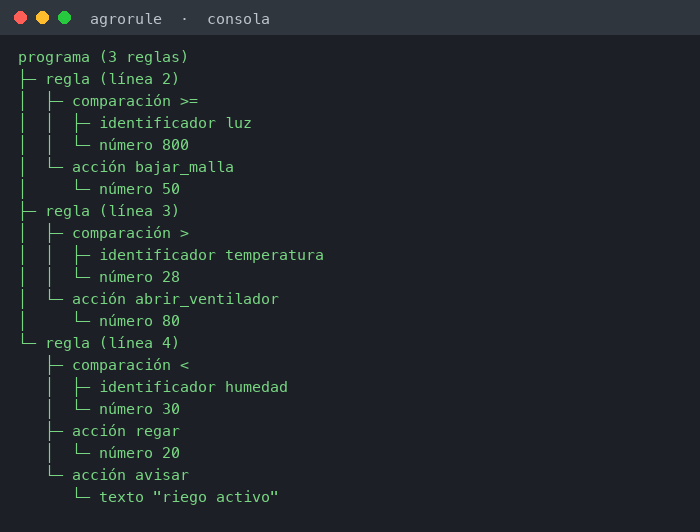
\includegraphics[width=0.60\textwidth]{figuras/captura_valido.png}\\[3pt]
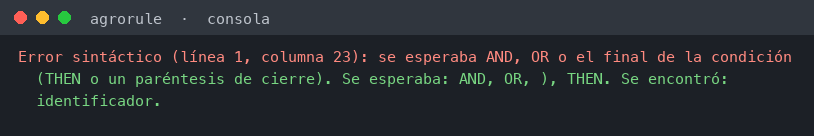
\includegraphics[width=0.70\textwidth]{figuras/captura_error.png}
\caption{Demostración: análisis de tres reglas válidas (arriba) y error localizado por ausencia de THEN (abajo).}\label{fig:demo}
\end{figure}
\end{document}
